\subsection{Разработка алгоритма работы с программным средством}
\label{sec:design:app}

Алгоритм работы программного средства представлен на рисунке~\ref{fig:design:app:diagram}.
При входе в приложение открывается пользователю должен предоставляться выбор списка сущностей, с которыми он может работать (также возможно отображение одно из списков по умолчанию с возможностью перехода к остальным).
Как видно из рисунка~\ref{fig:design:app:diagram} за взаимодействие с пользователем отвечают три основных модуля: модуль работы с транзакциями, модуль работы со счетами и модуль работы с категориями.

Стоит отметить некоторые особенности приложения с точки зрения взаимодействия с пользователем:
\begin{itemize}
    \item Основу проектируемого приложения предполагается расположить трёх главных формах (экранах), каждая из которых отвечает за взаимодействие с конкретным логическим модулем.
    \item Операции по созданию новых сущностей должны осуществляться через отдельные элементы управления, по модификации существующих данных -- через работу с элементами списков.
    \item Сводные значения по счетам отображаются на той же форме, что и список счетов.
    \item После каждой операции с данными соответствующий список должен обновляться.
    \item Операция создания денежного перевода осуществляется через выбор счёта-отправителя из списка существующих счетов.
    \item При удалении категории требуется дополнительный выбор политики удаления зависимых транзакций.
\end{itemize}

\begin{sidewaysfigure}
    \centering
    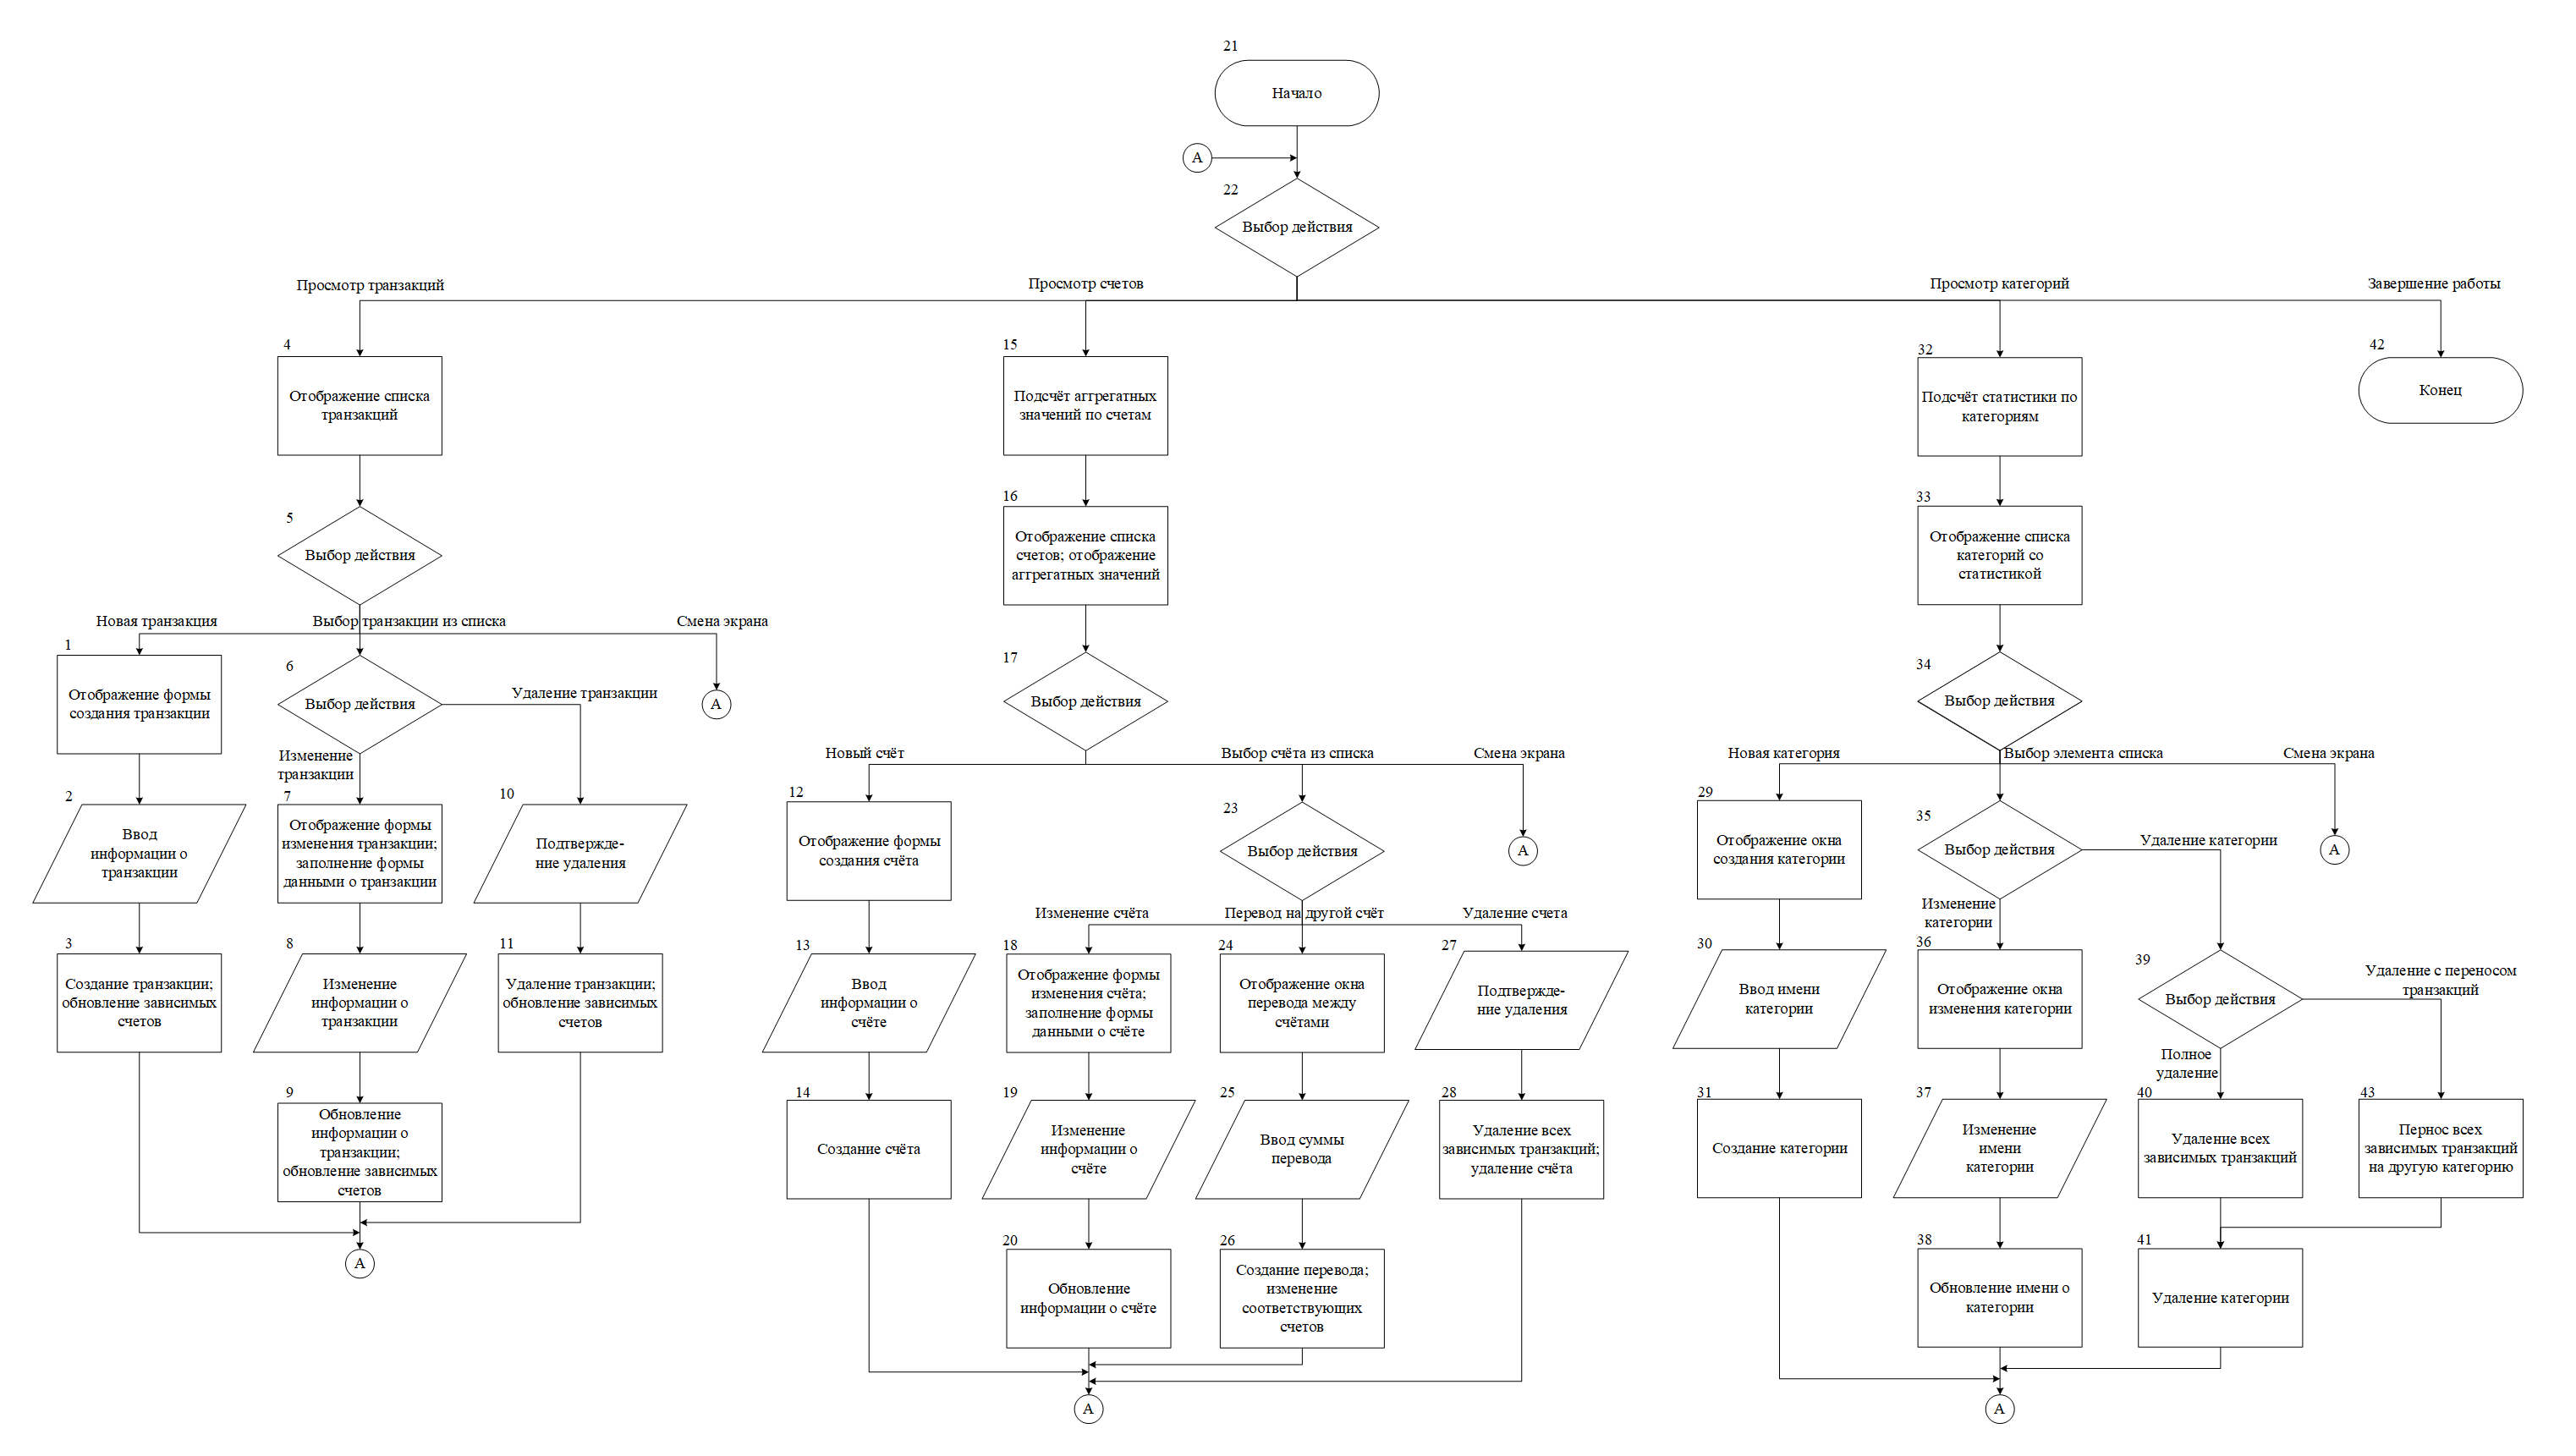
\includegraphics[scale=0.3]{3_4_app_diagram.png}
    \caption{Схема программного средства}
    \label{fig:design:app:diagram}
\end{sidewaysfigure}

